\documentclass[./main.tex]{subfiles}

\begin{document}

\subsection*{你好递归!}

递归对于 Haskell 而言很重要,因为不同于其他命令式语言,Haskell 中的计算是通过声明某物,而不是声明如何获取。这就是为什么 Haskell 中
没有 while 循环以及 for 循环,取而代之的则是递归。

\subsection*{Maximum}

\acode{maximum}函数接受一组可排序的列表(例如\acode{Ord} typeclass 的实例),并返回它们之间最大的那个。

现在让我们看一下如何递归的实现这个函数。我们首先可以确立一个边界条件,同时声明该列表的最大值等同于列表中的唯一元素,接着声明如果头大于尾时
长列表的头是最大值,如果尾更大那么继续上述过程:

\begin{lstlisting}[language=Haskell]
  maximum' :: (Ord a) => [a] -> a
  maximum' [] = error "maximum of empty list"
  maximum' [x] = x
  maximum' (x : xs)
    | x > maxTail = x
    | otherwise = maxTail
    where
      maxTail = maximum' xs
\end{lstlisting}

如上所示,模式匹配与递归非常的相配!大多数命令式语言并没有模式匹配,因此需要编写一堆 if else 声明来测试边界条件。而 Haskell 中仅需令
它们成为模版。这里使用了\textit{where}绑定来定义\acode{maxTail}作为列表尾的最大值。

\begin{figure}[h]
  \centering
  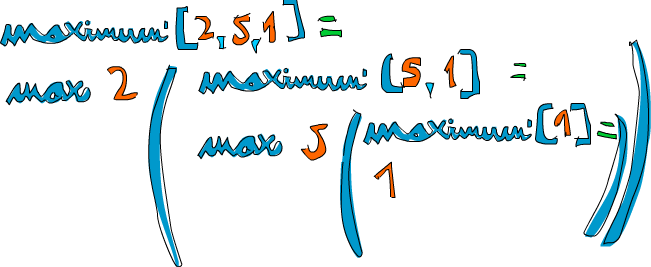
\includegraphics[width=0.9\textwidth]{\subfix{./images/maxs.png}}
\end{figure}

\subsection*{更多的递归函数}

让我们使用递归再来实现一些函数。首先是\acode{replicate},接受一个\acode{Int}以及一些元素,返回一个列表拥有若干重复的元素。

\begin{lstlisting}[language=Haskell]
  replicate' :: (Num i, Ord i) => i -> a -> [a]
  replicate' n x
    | n <= 0 = []
    | otherwise = x : replicate' (n - 1) x
\end{lstlisting}

这里使用守护而不是模式是因为需要测试一个布尔值条件。

\begin{anote}
  \acode{Num}并不是\acode{Ord}的子类,也就是说一个数值的组成并不依赖于排序。这就是为什么在做加法或减法或比较时,需要同时指定
  \acode{Num}与\acode{Ord}的类约束。
\end{anote}

接下来是实现\acode{take}:

\begin{lstlisting}[language=Haskell]
  take' :: (Num i, Ord i) => i -> [a] -> [a]
  take' n _
    | n <= 0 = []
  take' _ [] = []
  take' n (x : xs) = x : take' (n - 1) xs
\end{lstlisting}

注意这里使用了\acode{_}来匹配列表,因为我们并不关心列表里面的情况;同时,我们使用了一个守护,但是并没有\acode{otherwise}部分,
这意味着如果\acode{n}大于 0 的情况下,匹配将会失败并跳转到下一个匹配。第二个匹配指明如果尝试从空列表中提取任何元素,返回空列表。
第三个模式将一个列表分割成一个头与一个尾,接着将从一个列表中获取\acode{n}个元素相等于拥有\acode{x}头与一个尾视作一个列表获取
\acode{n-1}元素。

\begin{lstlisting}[language=Haskell]
  take' :: (Num i, Ord i) => i -> [a] -> [a]
  take' n _
    | n <= 0 = []
  take' _ [] = []
  take' n (x : xs) = x : take' (n - 1) xs
\end{lstlisting}

接下来是\acode{reverse}函数:

\begin{lstlisting}[language=Haskell]
  reverse' :: [a] -> [a]
  reverse' [] = []
  reverse' (x : xs) = reverse' xs ++ [x]
\end{lstlisting}

由于 Haskell 支持无线列表,\acode{reverse}并没有一个真正的边界检查,但是如果不这么做,那么则会一直计算下去或者生产出一个无限的
数据结构,类似于无限列表。无限列表的好处是我们可以在任意处进行截断。然后是\acode{repeat}函数,其返回一个无限列表:

\begin{lstlisting}[language=Haskell]
  repeat' :: a -> [a]
  repeat' x = x:repeat' x
\end{lstlisting}

接下来是\acode{zip}函数:

\begin{lstlisting}[language=Haskell]
  zip' :: [a] -> [b] -> [(a, b)]
  zip' _ [] = []
  zip' [] _ = []
  zip' (x : xs) (y : ys) = (x, y) : zip' xs ys
\end{lstlisting}

最后一个是\acode{elem}函数:

\begin{lstlisting}[language=Haskell]
  elem' :: (Eq a) => a -> [a] -> Bool
  elem' a [] = False
  elem' a (x : xs)
    | a == x = True
    | otherwise = a `elem'` xs
\end{lstlisting}

\newpage

\subsection*{快排!}

这里是主要算法:\textbf{排序列表是这样的一个列表,它包含所有小于(或等于)前面的列表头的值(这些值都是排序过的),然后是中间的列表头
  然后是所有大于列表头的值(它们也是排序过的)}。注意定义中两次提到了\textit{排序},那么我们将进行两次递归!同样也注意我们使用的是动词
\textit{is}在算法中进行定义,而不是\textit{做这个,做那个,再做另一个...}这就是函数式编程的魅力:

\begin{lstlisting}[language=Haskell]
  quicksort :: (Ord a) => [a] -> [a]
  quicksort [] = []
  quicksort (x:xs) =
    let
      smallerSorted = quicksort [a | a <-xs, a <= x]
      biggerSorted = quicksort [a|a<- xs, a>x]
    in
      smallerSorted ++ [x] ++ biggerSorted
\end{lstlisting}

测试:

\begin{lstlisting}[language=Haskell]
  ghci> quicksort [10,2,5,3,1,6,7,4,2,3,4,8,9]
  [1,2,2,3,3,4,4,5,6,7,8,9,10]
  ghci> quicksort "the quick brown fox jumps over the lazy dog"
  "        abcdeeefghhijklmnoooopqrrsttuuvwxyz"
\end{lstlisting}

\begin{figure}[h]
  \centering
  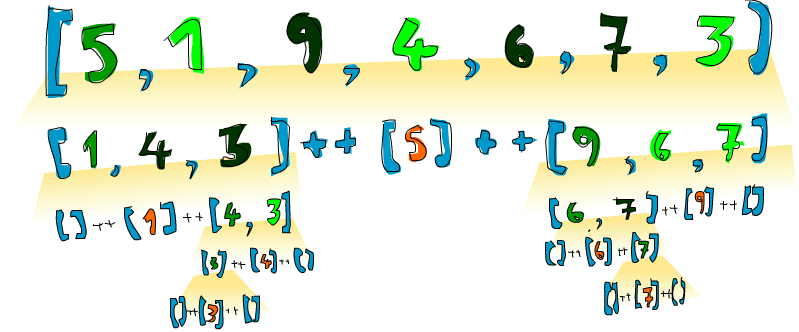
\includegraphics[width=0.9\textwidth]{\subfix{./images/quicksort.png}}
\end{figure}

\end{document}
